\documentclass[a4 paper]{article}
\usepackage[inner=2.0cm,outer=2.0cm,top=2.5cm,bottom=2.5cm]{geometry}
\usepackage{setspace}
\usepackage[ruled]{algorithm2e}
\usepackage[rgb]{xcolor}
\usepackage{verbatim}
\usepackage{subcaption}
\usepackage{amsgen,amsmath,amstext,amsbsy,amsopn,tikz,amssymb}
\usepackage{fancyhdr}
\usepackage[colorlinks=true, urlcolor=blue,  linkcolor=blue, citecolor=blue]{hyperref}
\usepackage[colorinlistoftodos]{todonotes}
\usepackage{rotating}
\usepackage{booktabs}
\newcommand{\ra}[1]{\renewcommand{\arraystretch}{#1}}

\newtheorem{thm}{Theorem}[section]
\newtheorem{prop}[thm]{Proposition}
\newtheorem{lem}[thm]{Lemma}
\newtheorem{cor}[thm]{Corollary}
\newtheorem{defn}[thm]{Definition}
\newtheorem{rem}[thm]{Remark}
\numberwithin{equation}{section}

\newcommand{\homework}[6]{
	\pagestyle{myheadings}
	\thispagestyle{plain}
	\newpage
	\setcounter{page}{1}
	\noindent
	\begin{center}
		\framebox{
			\vbox{\vspace{2mm}
				\hbox to 6.28in { {\bf MATH 118:~Statistics and Probability \hfill {\small (#2)}} }
				\vspace{6mm}
				\hbox to 6.28in { {\Large \hfill #1  \hfill} }
				\vspace{6mm}
				\hbox to 6.28in { {\it Instructor: {\rm #3} \hfill Name: {\rm #5} \hfill Student Id: {\rm #6}} \hfill}
				\hbox to 6.28in { {\it Assistant: #4  \hfill #6}}
				\vspace{2mm}}
		}
	\end{center}
	\markboth{#5 -- #1}{#5 -- #1}
	\vspace*{4mm}
}

\newcommand{\problem}[2]{~\\\fbox{\textbf{Problem #1}}\hfill (#2 points)\newline\newline}
\newcommand{\subproblem}[1]{~\newline\textbf{(#1)}}
\newcommand{\D}{\mathcal{D}}
\newcommand{\Hy}{\mathcal{H}}
\newcommand{\VS}{\textrm{VS}}
\newcommand{\solution}{~\newline\textbf{\textit{(Solution)}} }

\newcommand{\bbF}{\mathbb{F}}
\newcommand{\bbX}{\mathbb{X}}
\newcommand{\bI}{\mathbf{I}}
\newcommand{\bX}{\mathbf{X}}
\newcommand{\bY}{\mathbf{Y}}
\newcommand{\bepsilon}{\boldsymbol{\epsilon}}
\newcommand{\balpha}{\boldsymbol{\alpha}}
\newcommand{\bbeta}{\boldsymbol{\beta}}
\newcommand{\0}{\mathbf{0}}

\usepackage{listings}
\usepackage{color}

\definecolor{dkgreen}{rgb}{0,0.6,0}
\definecolor{gray}{rgb}{0.5,0.5,0.5}
\definecolor{mauve}{rgb}{0.58,0,0.82}

\lstset{frame=tb,
  language=Java,
  aboveskip=3mm,
  belowskip=3mm,
  showstringspaces=false,
  columns=flexible,
  basicstyle={\small\ttfamily},
  numbers=none,
  numberstyle=\tiny\color{gray},
  keywordstyle=\color{blue},
  commentstyle=\color{dkgreen},
  stringstyle=\color{mauve},
  breaklines=true,
  breakatwhitespace=true,
  tabsize=3
}


\begin{document}
	\homework{Homework \#2}{Due: 07/06/21}{Dr. Zafeirakis Zafeirakopoulos}{Gizem S\"ung\"u}{Ömer Faruk Bitikçioğlu}{161044010}
	\textbf{Course Policy}: Read all the instructions below carefully before you start working on the assignment, and before you make a submission.
	\begin{itemize}
		\item It is not a group homework. Do not share your answers to anyone in any circumstance. Any cheating means at least -100 for both sides. 
		\item Do not take any information from Internet.
		\item No late homework will be accepted. 
		\item For any questions about the homework, send an email to gizemsungu@gtu.edu.tr.
		\item Submit your homework (both your latex and pdf files in a zip file) into the course page of Moodle.
		\item Save your latex, pdf and zip files as "Name\_Surname\_StudentId".\{tex, pdf, zip\}.
		\item The answer which has only calculations without any formula and any explanation will get zero. 
		\item The deadline of the homework is 07/06/20 23:55.
		\item I strongly suggest you to write your homework on \LaTeX. However, hand-written paper is still accepted \textbf{IFF} your hand writing is \textbf{clear and understandable to read}, and the paper is well-organized. Otherwise, I cannot grade your homework.
		\item You do not need to write your Student Id on the page above. I am checking your ID from the file name.
	\end{itemize}
	
	\problem{1:}{10+10+10+10+10+10+40 = 100}
	\textbf{WARNING:} Please show your OWN work. Any cheating can be easily detected and will not be graded.
	\newline
	\newline
	For the question, please follow the file called manufacturing\_defects.txt while reading the text below.\\
	\newline
	In each year from 2000 to 2019, the number of manufacturing defects in auto manufacturers were counted. The data was collected from 14 different auto manufactory companies. The numbers of defects for the companies are indicated in 14 columns following the year column. Assume that the number of manufacturing defects per auto company per year is a random variable having a Poisson($\lambda$) and that the number of defects in different companies or in different years are independent.\\
	(Note: You should implement a code for your calculations for each following subproblem. You are free to use any programming languages (Python, R, C, C++, Java) and their related library.)
	
	\subproblem{a} Give a table how many cases occur for all companies between 2000 and 2019 for each number of defects (\# of Defects).\\
	Hint: When you check the file you will see: \# of Defects = \{0, 1, 2, 3, 4\}.\\
	\begin{table}[htb!]
		\centering
		\begin{tabular}{c|c}
			\begin{tabular}[c]{@{}c@{}}\textbackslash{}\# of\\Defects\end{tabular} & \begin{tabular}[c]{@{}c@{}}\textbackslash{}\# of cases\\in all company \\between the years\end{tabular}  \\ 
			\hline
			0                                                                      &                      144                                                                                    \\
			1                                                                      &                         91                                                                                 \\
			2                                                                      &                            32                                                                              \\
			3                                                          & 11
			\\
			4                                                                      & 2                                                                                                       
		\end{tabular}
		
		\caption{Actual cases}
		\label{tab1}
	\end{table}
	
	\subproblem{b} Estimate $\lambda$ from the given data. \\
$\lambda$ = 0.7
	\subproblem{c} Update Table \ref{tab1} in Table \ref{tab2} with Poisson predicted cases with the estimated $\lambda$.\\
	\begin{table}[htb!]
		\centering
		\begin{tabular}{c|c|c}
			\begin{tabular}[c]{@{}c@{}}\textbackslash{}\# of\\Defects\end{tabular} & \begin{tabular}[c]{@{}c@{}}\textbackslash{}\# of cases\\in all companies\\between the years\end{tabular} & \begin{tabular}[c]{@{}c@{}}Predicted \textbackslash{}\# of cases\\in all companies\\between the years\end{tabular}  \\ 
			\hline
			0                                                                      &                144                                                                                          &                                                                                                                    139,043885 \\
			1                                                                      &                      91                                                                                    &                                                                                                                    97,330720 \\
			2                                                                      &                        32                                                                                  &                                                                                                                     34,065752 \\
			3                                                                      &                        11                                                                                  &    7,948675
			\\
			4                                                                      &                         2                                                                                 &                                                                                                                   1,391018
		\end{tabular}
		\caption{Actual vs. Predicted Cases}
		\label{tab2}
	\end{table}
	\subproblem{d} Draw a barplot for the actual cases (Table \ref{tab2} in column 2) and the predicted cases (Table \ref{tab2} column 3) with respect to \# of defecrs. You should put the figure.\\
	
	
	\subproblem{e} According to the barplot in (c), does the poisson distribution fit the data well? Compare the values of the actual cases and the values of the poisson predicted cases, and write your opinions about performance of the distribution.\\
	Actual cases and predicted values are perfectly fit. Some predictions are a bit below of the actual cases, some of them a bit above the actual ones but they are very close that we can say the distribution is working well.
	\subproblem{f} According to your estimations above, write your opinions considering your barplot and Table \ref{tab2}. Which company do you prefer to buy a car? Why?\\
	Most of the time the possibility of a defect happens is very rare. Bu it is not imposibble. It can happen time to time. So, we can not say cars are very safe to use. A defection can cause fatal injuries, so it is a big problem to be honest.
	\subproblem{g} Paste your code that you implemented for the subproblems above. Do not forget to write comments on your code.\\
	\begin{itemize}
		\item The common code block for all subproblems\\
		\begin{lstlisting}
    private static final int MAX_DEFECT = 4;
    private static final int TIME = 20;
    private static final int NUM_OF_COMPANIES = 14;

    /**
     * Find the factorial of given number
     * @param num the number to be processed
     * @return the factorial of the given number
     */
    private static double fact(int num) {
        if (num < 0) {
            throw new InvalidParameterException();
        }
        int result = 1;
        for (int mult = 2 ; mult <= num; ++mult) {
            result = result * mult;
        }
        return result;
    }
		\end{lstlisting}
		\item The code block for (a)\\
		\begin{lstlisting}
/**
     * Calculates and returns the total number of actual cases
     * for each defect.
     * @return the number of actual cases for each defect
     */
    private static int[] giveCases() {
        try {
            BufferedReader br = new BufferedReader(new FileReader("manufacturing_defects.txt"));
            String line = br.readLine();
            int[] cases = new int[MAX_DEFECT+1];
            while (line != null) {
                String[] row = line.split("\t");
                // Count the number of cases for all companies and all years
                // for each number of defects (# of defects -> 0,1,2,3,4)
                for (int i = 2; i < row.length; ++i) {
                    int index = Integer.parseInt(row[i]); // 0,1,2,3 or 4
                    cases[index]++;
                }
                line = br.readLine();
            }
            br.close();
            return cases;
        } catch (IOException e) {
            e.printStackTrace();
        }
        return null;
    }
		\end{lstlisting}
		\item The code block for (b)\\
		\begin{lstlisting}
/**
     * Calculates the lambda according to the given data
     * @return the lambda value
     */
    private static double estimateLambda() {
        double lambda = 0.0;
        try {
            BufferedReader br = new BufferedReader(new FileReader("manufacturing_defects.txt"));
            String line = br.readLine();
            while (line != null) {
                String[] row = line.split("\t");
                double total = 0.0;
                for (int i = 2; i < row.length; ++i) {
                    total += Integer.parseInt(row[i]);
                }
                lambda += total / NUM_OF_COMPANIES; // Calculate the mean for each year
                line = br.readLine();
            }
            br.close();
        } catch (IOException e) {
            e.printStackTrace();
        }
        lambda /= TIME; // Calculate the mean for all years
        return lambda;
    }
		\end{lstlisting}
		\item The code block for (c)\\
		\begin{lstlisting}
/**
     * Calculates and returns the predicted case values.
     * Uses Poisson distribution to calculate the predictions.
     * @param totalCase the number of total cases for all the time
     * @param lambda the lambda value
     * @return the predicted case values
     */
    private static double[] findPredictions(int totalCase, double lambda) {
        double[] predictions = new double[MAX_DEFECT+1];
        double negLambda = (-1) * lambda;
        for (int i = 0; i <= MAX_DEFECT; ++i) {
            predictions[i] = ((Math.exp(negLambda) * Math.pow(lambda, i)) / fact(i)) * totalCase;
        }
        return predictions;
    }
		\end{lstlisting}
		\item The code block for (d)\\
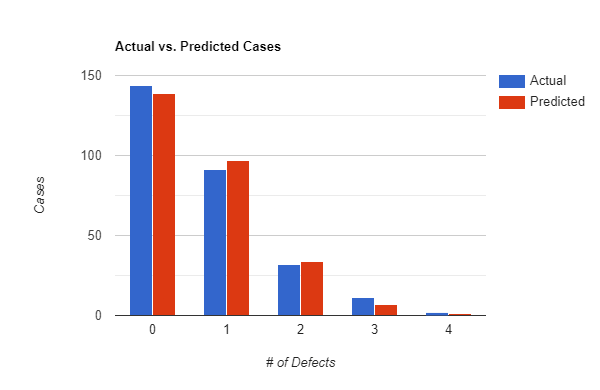
\includegraphics[width=\textwidth]{C:/Users/OFB/Desktop/Omer_Bitikcioglu_161044010/actual_vs_predicted.png}


	\end{itemize}
	
	
	
	
\end{document} 


